\section{INTRODUCTION} % (fold)
\label{sec:introduction}
	The purpose of this report is to analyze inefficiencies, bottlenecks and the removal of these issues from KDb and its querying syntax.
	
	\subsection{Background} % (fold)
	\label{sub:background}
Kdb+ is a relatively new product, released in 2003 by the company Kx, that was specially designed to meet the needs of lead-edge real-time businesses. Kdb+ is an in-memory column-oriented database system that is designed to capture, analyze, compare and store data while maintaining high execution speeds on high volumes of data. \cite{FAQ}  Traditional database systems divide real-time(front-end) data and historical(back-end) data.  The real-time data is used to make current business decisions and historical data is used to test new strategies before releasing them.  Until the recent boom in data-collection by different companies, the traditional method was sufficient.  However, with the recent growth in the data each company needs to collect and analyze, this was no longer acceptable.  Kx architected the kdb+ system to have no split between how real-time and historical data is handled and analyzed.  This allows for instant analysis of incoming data as well as comparisons of that streaming data with historical data - something that was not previously possible with other database solutions.\\

Although kdb+ was specifically designed for these reasons, each implementation of kdb+ is different for each company.  There are a number of issues with the actual hardware implementation such as
	\begin{enumerate}
		\item[a)] the amount of available RAM
		\item[b)] swap space
		\item[c)] hard drive setup
		\item[d)] how the data is stored
	\end{enumerate}
that significantly affects the performance and efficiency of the database system as a whole. The cause of the inefficiency or bottleneck and possible solutions will be discussed in this report.\\

Kdb+ comes with this own, specially designed, querying language named Q. The Q language is based off of the same K programming language that kdb+ itself is developed off of.  In addition to querying capabilities, it also allows for complex programming as K is a programming language.  Traditionally, databases would have APIs for Java or C++ so that programs could be designed to manipulate and analyze data.  The querying language for those traditional databases were only for querying and nothing else.  Since programming is possible in Q directly, this is much more efficient than other systems because it was designed to interact directly with the database structure, something that is not possible with Java or C++.  Q also allows for extremely efficient processing and retrieval of data because it was designed to execute each command or query in bulk instead of on each individual record (row) in a table of the database.  Although Q is a very powerful language, its uses and the language in general is not well documented and it is extremely difficult to learn and fully utilize even some basic features for that reason.  There are also many common mistakes that even seasoned developers for the Q language make and this report will discuss many of these.\\
	% subsection background (end)

	\subsection{Scope} % (fold)
	\label{sub:scope}
This report analyzes implementation issues of kdb+ for both aspects of hardware and software. While there are many possible ways to customize and set up a kdb+ system, for the purpose of this report only the most typical setup will be considered.\\ 
\begin{figure}[htp]
	\centering
	\subfigure{}
	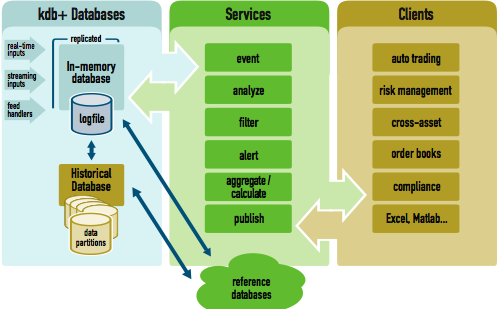
\includegraphics[width=.80\textwidth]{images/conceptual}
	\caption[kdb+ Diagram]{Typical kdb+ implementation discussed in this report\cite{whitepaper}}
	\label{fig:typical kdb+ system}
\end{figure}\\

From the diagram above, a typical kdb+ implementation consists of the hardware the database runs off of, the software services that interface with the database and the front-end clients that use the the software services to display the information in a meaningful manner.  This report disregards the last section of the kdb+ implementation and will only discuss the kdb+ Databases and services layers labeled labeled in the diagram.  Thus any reference ``hardware'' in this report refers to the physical kdb+ databases and any reference to ``software'' refers to the services layer used to interface with the front-end. The physical kdb+ databases will also be more commonly referred to as a ``server'' and this can be narrowed down into a simple computer with multiple cores (in this case, four) and sufficient RAM (eight to sixteen gigabytes).  Lastly, all references to the ``system'' refer to the implementation as a whole and encompasses all three layers of the diagram above.\\
	% subsection scope (end)

	\subsection{Outline} % (fold)
	\label{sub:outline}
There are two sections in this report that analyze different issues with certain aspects of the hardware and software layers of a kdb+ system.  Each section will analyze an issue and discuss a possible solution for that issue.  Lastly, there will be a section on the benefits - many of which are not readily apparent - that these changes will bring.  Throughout the report, a variety of terms are used so a glossary of terms has been included for reference. The first section of the report discusses some issues with the hardware implementation.  These issues include ``RAM'', ``Allocation of Swap Space'', ``Hard Drives - Space and Quantity'', ``Partitioned Tables''.  The second section of this report pertains to software issues and gives a number of examples of incorrect usage of the Q programming language and analyses how these issues affect the integrity of the kdb+ system as a whole.  Methods of avoiding these issues and methods of improving the system from a software perspective are discussed.
	% subsection outline (end)

% section introduction (end)
